Se utilizó el algoritmo \textbf{KMeans} de la librería \textbf{Scikit Learn} \autocite{scikit-learn} con la utilización de sus parámetros por defecto \autocite{sklearn\_api}. Al tratarse de un método sin supervisión necesitamos indicarle la cantidad de clusters en las cuales se quiere que estén agrupadas las observaciones.

Para medir que tan "bien" resulta la agrupación vamos a utilizar diferentes medidas. La primera para identificar cual será la cantidad de clusters será utilizar la suma de los errores cuadrados medios, o \textbf{SSE} por sus siglas en inglés. También nos apoyaremos en la medida de \textbf{silhouette} para observar que cantidad de clusters obtuvo el mejor valor y también para validar la consistencia de los clusters obtenidos. Como métrica adicional para validar la consistencia de los grupos generados \textbf{Rand index}.

Comenzaremos con generar entre 2 a 6 clusters para los atributos de alto nivel, luego elegida la cantidad de clusters vamos a proceder a agrupar las mismas canciones pero utilizando los datos de bajo nivel, recordar que usaremos las 4 medidas que resumen la información y obtuvimos en el trabajo previo. Con estos nuevos resultados se elegirá cual fue la medida que obtuvo mejores métricas y procederemos a concatenar los valores de alto nivel con esta última. Con este nuevo conjunto de generado vamos a recrear el experimento de generar de 2 a 6 clusters y observar si los resultados se repiten o no.
\subsection{Resultados}
\subsubsection{Atributos de alto nivel}
Vamos a comenzar analizando cual sería la mejor cantidad de clusters para los atributos de alto nivel.

\begin{figure}[H]
    \begin{subfigure}{.4\textwidth}
        \centering
        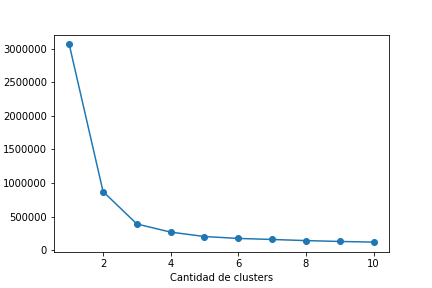
\includegraphics[width = 2in]{img/kmeans/elbow.png}
        \caption{Método elbow}
    \end{subfigure}
    \begin{subfigure}{.4\textwidth}
        \centering
        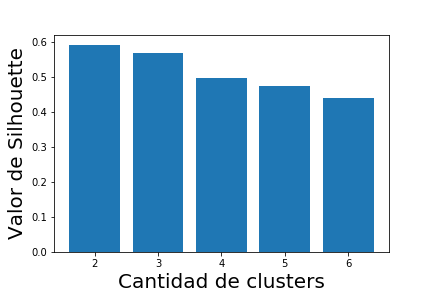
\includegraphics[width = 2in]{img/kmeans/silhouette-features.png}
        \caption{Silhouette score}
    \end{subfigure}
    \caption{Cantidad de clusters óptima}
    \label{fig:elbow-silhouette}
\end{figure}

Si solo tuviésemos en cuenta el método elbow podríamos elegir 4 clusters como el óptimo para realizar el agrupamiento pero, al observar los valores que se obtienen con el método del silhouette, se decidió que el número de clusters sea 3.

\begin{table}[H]
    \centering
    \begin{tabular}{|c|c|}
        \hline
        Cantidad de clusters & Indice de Rand \\
        \hline
        2 & 0.098 \\
        3 & 0.122 \\
        4 & 0.141 \\
        5 & 0.146 \\
        6 & 0.152 \\
        \hline
    \end{tabular}
    \caption{Rand index}
    \label{tab:rand-kmeans-af}
\end{table}

Para reforzar la elección de 3 como cantidad de clusters se puede apreciar que quitando un agrupamiento de 2 clusters, el resto de valores fue cambiando pero no tan abruptamente.

A continuación se muestra la tabla que se obtiene de evaluar los el método con 3 clusters en que grupo clasificó a cada pista musical.

\begin{table}[H]
    \centering
    \begin{tabular}{|c|c|c|c|}
        \hline
        & \multicolumn{3}{ c| }{Clusters} \\
        \hline
        Género & 0 & 1 & 2 \\
        \hline
        ambient & 224 & 58 & 178 \\
        classical & 253 & 32 & 120 \\
        drum-and-bass & 39 & 359 & 53 \\
        jazz & 159 & 56 & 212 \\
        world-music & 182 & 62 & 219 \\  
        \hline
    \end{tabular}
    \caption{Géneros musicales y grupos}
    \label{tab:cross-kmeans-af-3}
\end{table}

El género \textbf{drum-and-bass} es el que mejor concentración presenta en el cluster número 1, este mismo también presenta muy pocas observaciones del resto de los géneros musicales. Por último los clusters 0 y 2 contienen de forma balanceanda el resto de los géneros. Se podría sospechar que al menos para los atributos de alto nivel el género \textbf{drum-and-bass} se encuentra mas separado del resto de los estilos musicales. A modo de comparación vamos a incluir una tabla similar a ~\ref{tab:cross-kmeans-af-3} pero con 5 clusters. Y si observará el mismo comportamiento solo que esta vez el cluster 2 es quien concentra al estilo \textbf{drum-and-bass}.

\begin{table}[H]
    \centering
    \begin{tabular}{|c|c|c|c|c|c|}
        \hline
        & \multicolumn{5}{ c| }{Clusters} \\
        \hline
        Género & 0 & 1 & 2 & 3 & 4 \\
        \hline
        ambient & 90 & 124 & 43 & 106 & 97 \\
        classical & 52 & 157 & 28 & 77 & 91 \\
        drum-and-bass & 41 & 1 & 357 & 14 & 38 \\
        jazz & 86 & 57 & 48 & 136 & 100 \\
        world-music & 94 & 29 & 45 & 145 & 150 \\
        \hline
    \end{tabular}
    \caption{Géneros musicales y grupos}
    \label{tab:cross-kmeans-af-4}
\end{table}

\subsubsection{Atributos de bajo nivel}
En este caso ya decidimos que la cantidad de clusters serán 3, entonces para comenzar a evaluar que conjunto de medidas resúmenes (media y desvío estándar de timbres y pitches) es la más efectiva calculamos el valor de silhouette para cada uno de ellos.

\begin{figure}[H]
    \centering
    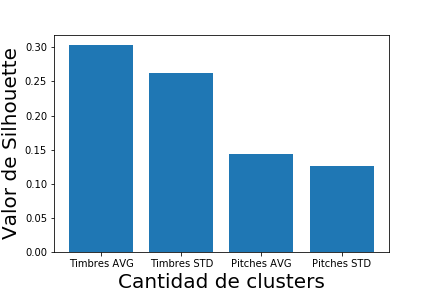
\includegraphics[width = 4in]{img/kmeans/silhouette-analysis.png}
    \caption{Silhouette}
    \label{fig:silhouette-aa-3-all}
\end{figure}

El pitch obtuvo valores muy bajos en comparación al timbre y de éste último vamos a explorar usando la medida de la media que obtuvo mejores valores. Adjuntamos la tabla con los valores del índice de Rand que refuerzan la elección ya que se obtuvieron valores muy superiores que con el resto de las medidas.

\begin{table}[H]
    \centering
    \begin{tabular}{|c|c|}
        \hline
        Conjunto de medidas resumenes & Indice de Rand \\
        \hline
        timbre y su media & 0.151 \\
        timbre y su desvío estándar & 0.084 \\
        pitch y su media & 0.096 \\
        pitch y su desvío estándar & 0.030 \\
        \hline
    \end{tabular}
    \caption{Rand index}
    \label{tab:rand-kmeans-aa-3-all}
\end{table}

Ahora analizaremos como fue realmente la clasificación según el estilo musical y comparar si los resultados fueron similares al trabajo realizado con los atributos anteriores.

\begin{table}[H]
    \centering
    \begin{tabular}{|c|c|c|c|}
        \hline
        & \multicolumn{3}{ c| }{Clusters} \\
        \hline
        Género & 0 & 1 & 2 \\
        \hline
        ambient & 224 & 197 & 39 \\
        classical & 237 & 86 & 82 \\
        drum-and-bass & 17 & 0 & 434 \\
        jazz & 246 & 42 & 138 \\
        world-music & 251 & 57 & 155 \\ 
        \hline
    \end{tabular}
    \caption{Géneros musicales y grupos}
    \label{tab:cross-kmeans-aa-3-avg-timbre}
\end{table}

De nuevo el género \textbf{drum-and-bass} fue el que mejor se clasificó en el cluster 2 dejando solo 17 elementos mal ubicados. Pero en comparación al otro conjunto de datos, éste clasificó más canciones en el mismo grupo que \textbf{drum-and-bass}, dejando al cluster 1 con muchos menos elementos que el resto.

\subsubsection{Unión de conjunto de datos}
A partir de las dos experimentaciones anteriores, se decidió unir el archivo de atributos de alto nivel con el promedio de los timbres. A partir de ésta mezcla vamos a realizar un estudio similar a los previamente realizados, comenzando por la elección del número de clusters.

\begin{figure}[H]
    \begin{subfigure}{.4\textwidth}
        \centering
        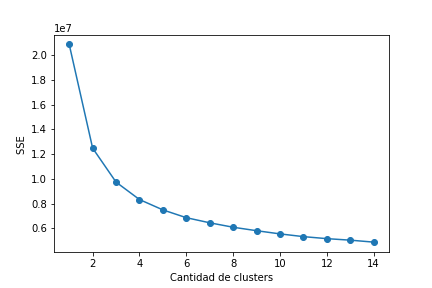
\includegraphics[width = 2in]{img/kmeans/elbow-join.png}
        \caption{Método elbow}
    \end{subfigure}
    \begin{subfigure}{.4\textwidth}
        \centering
        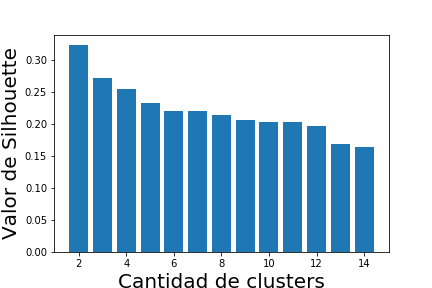
\includegraphics[width = 2in]{img/kmeans/silhouette-join.png}
        \caption{Silhouette score}
    \end{subfigure}
    \caption{Cantidad de clusters óptima}
    \label{fig:elbow-silhouette-join}
\end{figure}

En este caso se puede ver como la caída de la curva en el método elbow es mucho mas suave y no tan marcada como en el primer caso. Si bien parece que de nuevo 3 clusters sería el número ideal, también 4 o 5 obtuvieron buenos valores de silhouette. Vamos a elegir el número en 3 para poder compararlo con las experimentaciones previas y 4 para ver como se comporta contra el mismo conjunto de datos pero con la elección previa de 3 grupos. Siendo esta última unión la que mejores índices tiene y un valor muy superior cuando se eligen 4 grupos.

\begin{table}[H]
    \centering
    \begin{tabular}{|c|c|}
        \hline
        Conjunto de datos & Indice de Rand \\
        \hline
        Solo atributos alto nivel & 0.122 \\
        Solo atributos de bajo nivel & 0.151 \\
        Unión con 3 clusters & 0.186 \\
        Unión con 4 clusters & 0.245 \\
        \hline
    \end{tabular}
    \caption{Rand index}
    \label{tab:rand-kmeans-af-3-aa-3-join-3-join-4}
\end{table}

A continuación se puede apreciar como fueron ubicados las canciones en los diferentes grupos, primero con un número de clusters de 3 y luego de 4

\begin{table}[H]
    \centering
    \begin{tabular}{|c|c|c|c|}
        \hline
        & \multicolumn{3}{ c| }{Clusters} \\
        \hline
        Género & 0 & 1 & 2 \\
        \hline
        ambient & 219 & 22 & 219 \\
    	classical & 273 & 30 & 102 \\
    	drum-and-bass & 17 & 434 & 0 \\
    	jazz & 287 & 80 & 59 \\
    	world-music & 277 & 118 & 68 \\
        \hline
    \end{tabular}
    \caption{Géneros musicales en 3 grupos}
    \label{tab:cross-kmeans-join-3}
\end{table}

\begin{table}[H]
    \centering
    \begin{tabular}{|c|c|c|c|c|}
        \hline
        & \multicolumn{4}{ c| }{Clusters} \\
        \hline
        Género & 0 & 1 & 2 & 4 \\
        \hline
        ambient & 83 & 203 & 17 & 157 \\
		classical & 252 & 101 & 5 & 47 \\
		drum-and-bass & 8 & 0 & 427 & 16 \\
		jazz & 132 & 44 & 65 & 185 \\
		world-music & 77 & 52 & 98 & 236 \\
        \hline
    \end{tabular}
    \caption{Géneros musicales en 4 grupos}
    \label{tab:cross-kmeans-join-4}
\end{table}

De nuevo \textbf{drum-and-bass} al igual que en los previos experimentos resultó ser siempre el estilo más concentrado. Particularmente con la elección de 4 grupos se puede apreciar otras relaciones interesantes entre los estilo restantes. Por ejemplo en el cluster 0 hay muchos pistas del género \textit{classic} y \textit{jazz}, en el grupo 1 gran cantidad de \textit{ambient} y en último el número 3 se observa gran concentración de canciones del género \textit{classic} \textit{world-music}, \textit{jazz} y \textit{ambient}.

\begin{figure}[H]
    \begin{subfigure}{.4\textwidth}
        \centering
        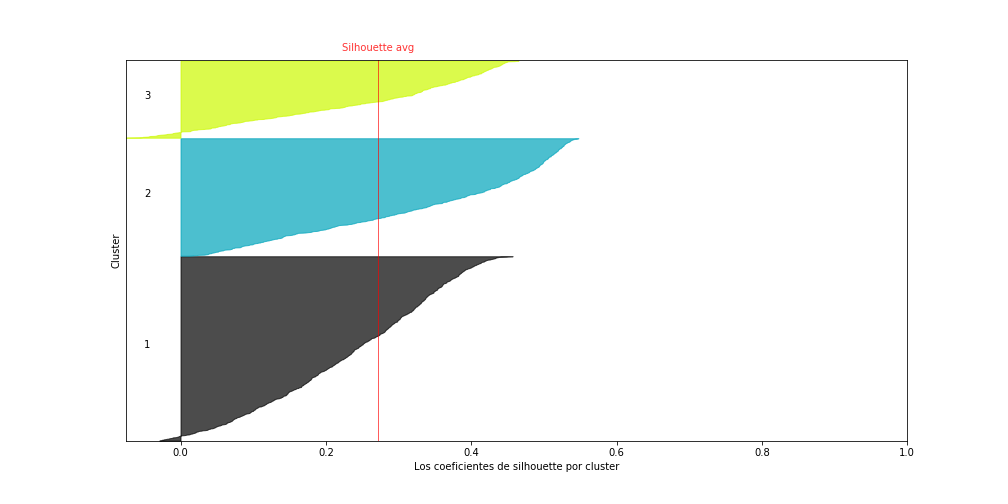
\includegraphics[width = 2in]{img/kmeans/silhouette-join-3-eo.png}
        \caption{Silhouette para 3 clusters}
    \end{subfigure}
    \begin{subfigure}{.4\textwidth}
        \centering
        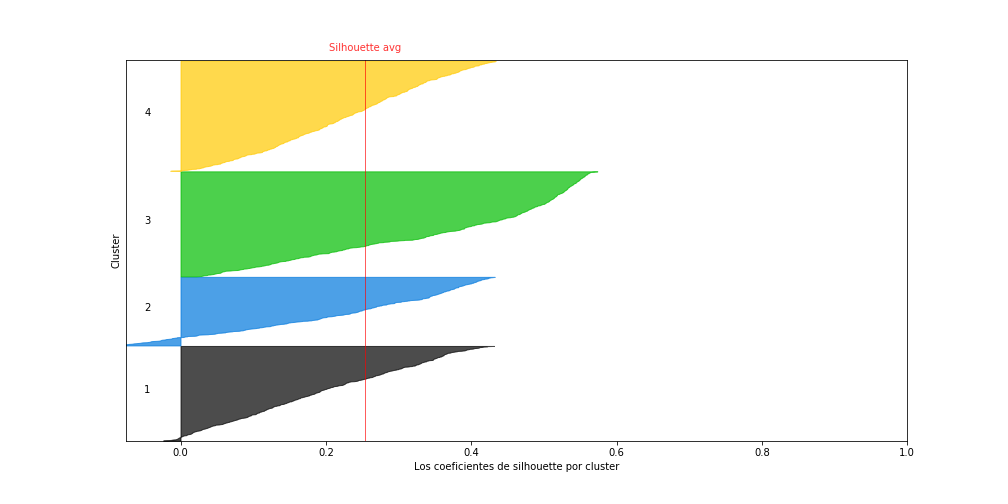
\includegraphics[width = 2in]{img/kmeans/silhouette-join-4-eo.png}
        \caption{Silhouette para 4 clusters}
    \end{subfigure}
    \caption{Silhouette en la unión de los atributos}
    \label{fig:silhouette-join-3-4}
\end{figure}

La elección de 4 clusters en este caso parece mucho más interesante ya que se comienzan a descubrir mejores relaciones y similitudes entre las canciones gracias a la unión de los datos.

Como se verá más adelante los valores obtenidos para éstas mismas métricas fueron superiores ya que se trata de métodos más complejos y que en general funcionan mejor. Es por eso que en este caso no se van a realizar más experimentos ni analizar métricas.

El algoritmo \textbf{KMeans} si bien no es el mejor y la implementación de \textit{Scikit Learn} no ofrece mucha parametría con la cuál experimentar, es muy útil para comenzar con cualquier tipo de análisis ya que es un método muy rápido que no requiere ningún tipo de supervisión y sirve como métrica con la cuál comparar al resto de los algoritmos.

